\documentclass[slovene,11pt,a4paper]{article}
%\usepackage{fullpage}

%dodatni paketki:
\usepackage{graphicx}
\usepackage{amsmath,amsfonts,amsthm} %matematicni paket
\usepackage{color} % omogoča barvno pisanje
\usepackage[utf8]
{inputenc}
\usepackage[slovene]{babel} % slovenski jezik/hyphenation
\usepackage{hyperref} %naredi vse povezave rečerenc, kazala,...
\numberwithin{equation}{section} % Number equations within sections (i.e. 1.1, 1.2, 2.1, 2.2 instead of 1, 2, 3, 4)
\numberwithin{figure}{section} % Number figures within sections (i.e. 1.1, 1.2, 2.1, 2.2 instead of 1, 2, 3, 4)
\numberwithin{table}{section} % Number tables within sections (i.e. 1.1, 1.2, 2.1, 2.2 instead of 1, 2, 3, 4)
\usepackage{eurosym} %za znak €

\usepackage[margin=2cm]{geometry}
\include{template}

\begin{document}
\begin{titlepage}

\newcommand{\HRule}{\rule{\linewidth}{0.5mm}} % Defines a new command for the horizontal lines, change thickness here

\center % Center everything on the page

%----------------------------------------------------------------------------------------
%	LOGO
%----------------------------------------------------------------------------------------

%\includegraphics{Logo}\\[1cm] % Include a department/university logo - this will require the graphicx package
 
%----------------------------------------------------------------------------------------


\includegraphics[width=2cm]{slike/aaa}\\[0.5cm]
 
%----------------------------------------------------------------------------------------
%	NASLOV DELA
%----------------------------------------------------------------------------------------
\textit{Univerza v Ljubljani}\\
\textit{Fakulteta za {\color{red}matematiko in fiziko}}\\[0.5cm]

\emph{Oddelek za fiziko}\\[0.5cm] % Oddelek za fiziko


%----------------------------------------------------------------------------------------
%	TITLE SECTION
%--------------------------------------------------------------------------------------
\HRule \\[0.4cm]
\huge {\bfseries 4. naloga: Populacijski model}\\[0.4cm] % NASLOV SEMINARJA
\HRule \\[0.5cm] 

 \textsc{\large Poročilo pri predmetu modelska analiza 1}\\
 \textsc{\large 2015/2016}\\[1cm] % SEMINASKO DELO
 
%----------------------------------------------------------------------------------------
%	AUTHOR SECTION
%----------------------------------------------------------------------------------------



% If you don't want a supervisor, uncomment the two lines below and remove the section above
\Large \emph{Avtor:}\\
Klemen \textsc{Rahne}\\
28152028\\[2cm]
%----------------------------------------------------------------------------------------
%	DATUM
%----------------------------------------------------------------------------------------

{\large \today } \\[0.5cm] % Date, change the \today to a set date if you want to be precise

	

\end{titlepage}


%----------------------------------------------------------------------------------------
%	KAZALO
%----------------------------------------------------------------------------------------

%\tableofcontents

%----------------------------------------------------------------------------------------
%	ZAČETEK TEKSTA
%----------------------------------------------------------------------------------------

\section{Zajci in lisice}

Zanima nas sprememba populacije zajcev in lisic v sistemu, kjer živijo le lisice in zajci. Modeliral, bom po naslednjih zakonitostih:
\begin{equation}
\begin{aligned}
\dot{Z}=\alpha Z-\beta Z L \\
\dot{L} = - \gamma L+\delta Z L
\end{aligned}
\end{equation}
pri čemer je $Z$, število zajce, $L$ število lisic, $\alpha, \beta, \gamma \text{ in } \delta$ parametri. Pika nad $Z,L$ označuje časovni odvod. Enačbi lahko preoblikujemo v brezdimenzijsko obliko:
\begin{equation}
\label{brezdim-osnovna-zajci}
\begin{aligned}
\dot{z}=\alpha z(1-l) \\
\dot{l} = \gamma l(z-1)
\end{aligned}
\end{equation}
Oglejmo si nekaj rešitev:
\begin{figure}[h]
\noindent\makebox[\textwidth][l]{%
\hspace{-\dimexpr\oddsidemargin+1in}%

\begin{minipage}[t]{0.5\paperwidth}
\begin{flushleft}

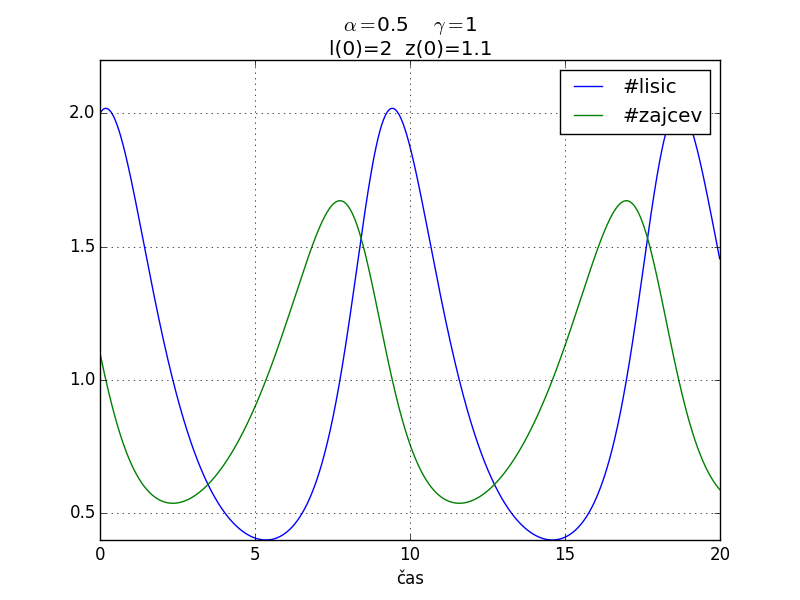
\includegraphics[scale=0.5]{slike/alfa0_5gama1l02z01_1.png}
\hspace{\fill}
\end{flushleft}
\end{minipage}
\begin{minipage}[t]{0.5\paperwidth}
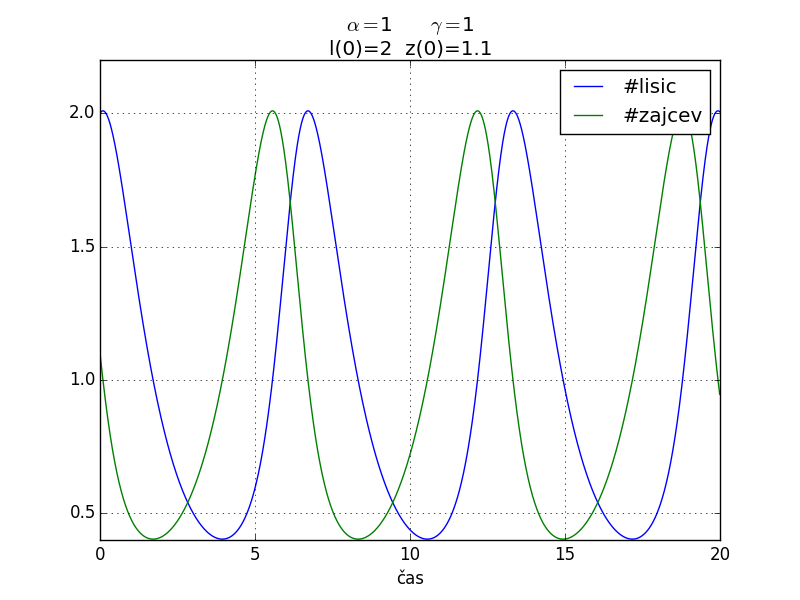
\includegraphics[scale=0.5]{slike/alfa1gama1l02z01_1.png}
\end{minipage}%
}
\noindent\makebox[\textwidth][l]{%
\hspace{-\dimexpr\oddsidemargin+1in}%

\begin{minipage}[t]{0.5\paperwidth}
\begin{flushleft}

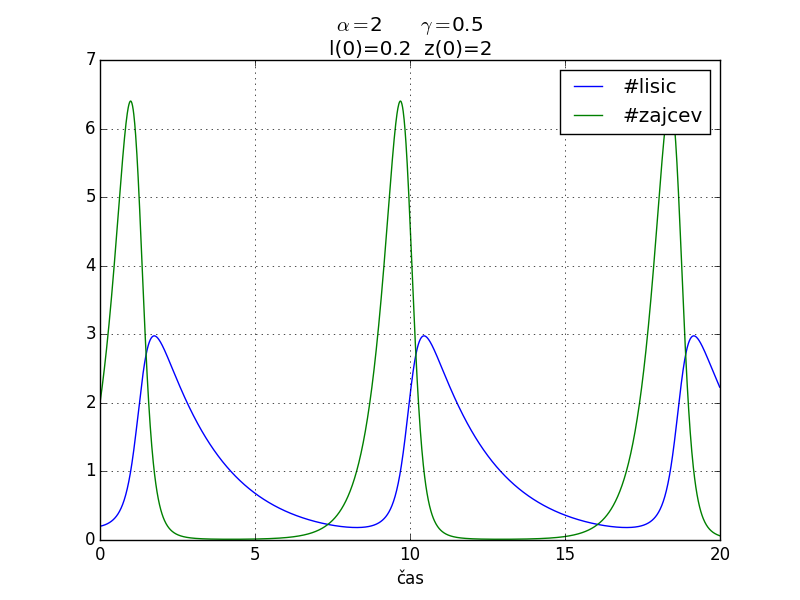
\includegraphics[scale=0.5]{slike/alfa2gama0_5l00_2z02.png}
\hspace{\fill}
\end{flushleft}
\end{minipage}
\begin{minipage}[t]{0.5\paperwidth}
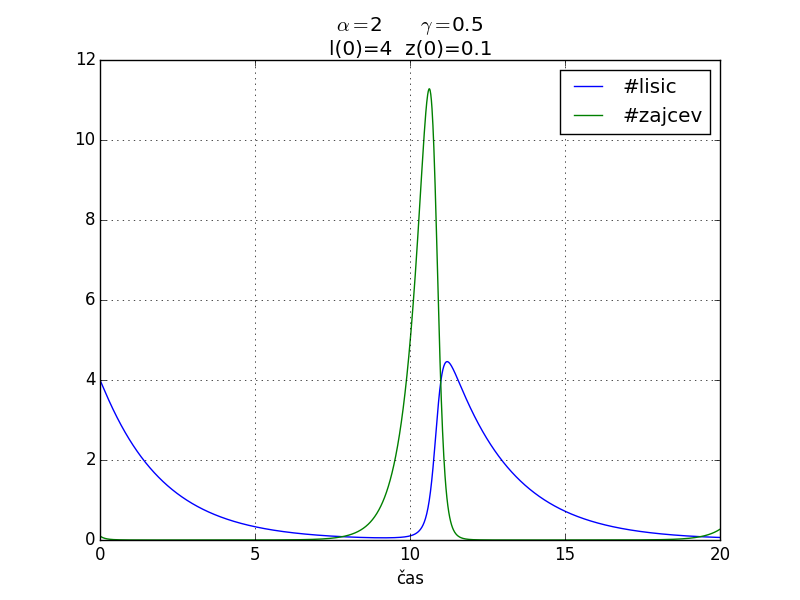
\includegraphics[scale=0.5]{slike/alfa2gama0_5l04z00_1.png}
\end{minipage}%
}
\caption{Primeri rešitev za nekaj različnih začetnih pogojih in parametrov.}
\end{figure}

\subsection{Stacionarne točke}
Oglejmo si še stacionarne točke. Iz enačbe \ref{brezdim-osnovna-zajci} sledi:

\begin{equation}
\label{brezdim-stacionarne-zajci}
\begin{aligned}
0=\dot{z}=\alpha z(1-l) \\
0=\dot{l} = \gamma l(z-1)
\end{aligned}
\end{equation}
Rešitev omenjenih enačb sta dve:
\begin{itemize}
\item $(z_1,l_1)=(0,0)$
\item $(z_2,l_2)=(1,1)$
\end{itemize}
Še grafa rešitve:

\begin{figure}[h]
\noindent\makebox[\textwidth][l]{%
\hspace{-\dimexpr\oddsidemargin+1in}%

\begin{minipage}[t]{0.5\paperwidth}
\begin{flushleft}

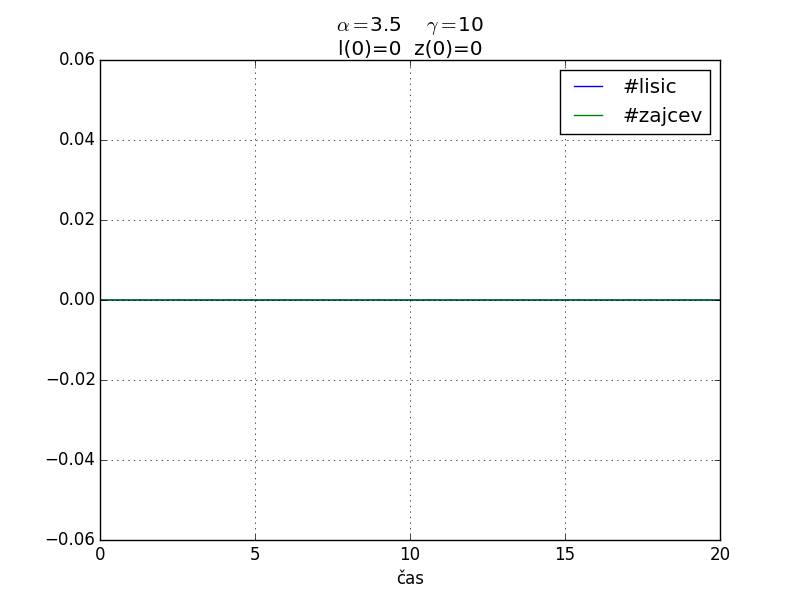
\includegraphics[scale=0.5]{slike/alfa3-5gama10l00z00.png}
\caption{Prva stacionarna točka}
\hspace{\fill}
\end{flushleft}
\end{minipage}
\begin{minipage}[t]{0.5\paperwidth}
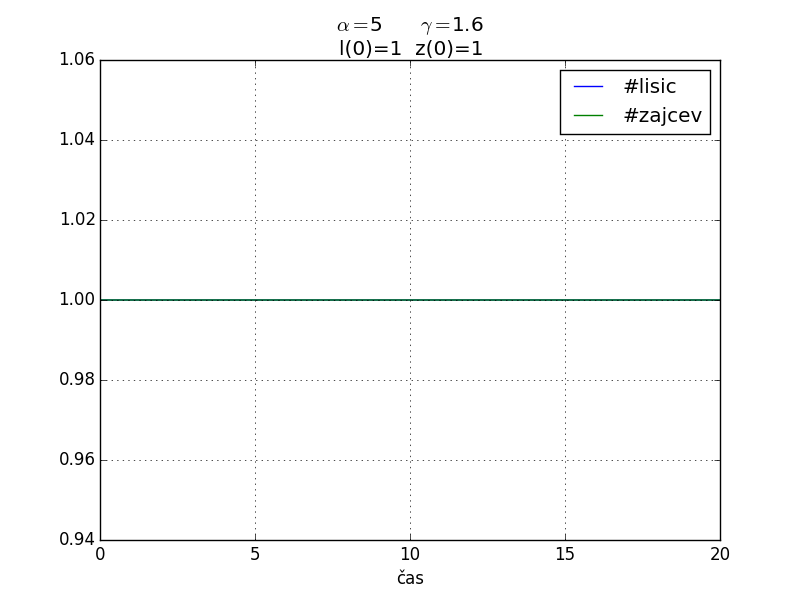
\includegraphics[scale=0.5]{slike/alfa5gama1-6l01z01.png}
\caption{Druga stacionarna točka}
\end{minipage}%
}
\end{figure}



V obeh primerih opazimo, da sta rešitvi neodvisni od parametra $\alpha$ in $\gamma$.
\subsection{Fazni diagram}
Oglejmo si še fazni diagram rešitev-odvisnost števila lisic proti številu zajcev. Vidimo, da se pri konstantnih vrednosti parametra $\alpha$ in $\gamma$ zaključene krivulje spreminjajo v obsegu. To je razumljivo, saj spreminjamo začetne vrednosti naših rešitev ("raztegujemo krivuljo").\\
V primeru spreminjanja parametra $\alpha$ in $\gamma$ in ohranjanju začetnih vrednosti števila zajcev in lisic, smo v faznem diagramu dobili elipse. V tem primeru se ohranjajo osi elips, spreminja pa se eliptičnost.

\begin{figure}[t!]
\noindent\makebox[\textwidth][l]{%
\hspace{-\dimexpr\oddsidemargin+1in}%

\begin{minipage}[t]{0.5\paperwidth}
\begin{flushleft}

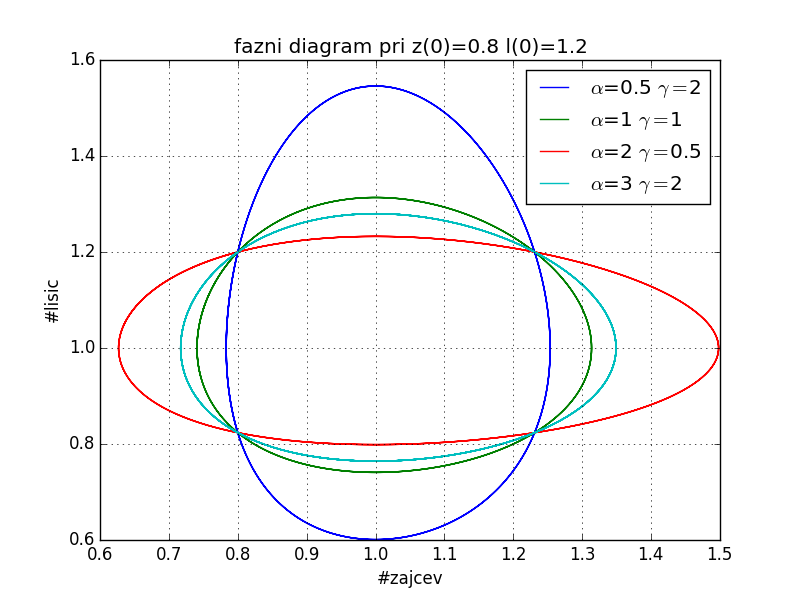
\includegraphics[scale=0.4]{slike/fazni-diagram-konstantni-zacetni-pogoji.png}
%\caption{Prva stacionarna točka}
\hspace{\fill}
\end{flushleft}
\end{minipage}
\begin{minipage}[t]{0.5\paperwidth}
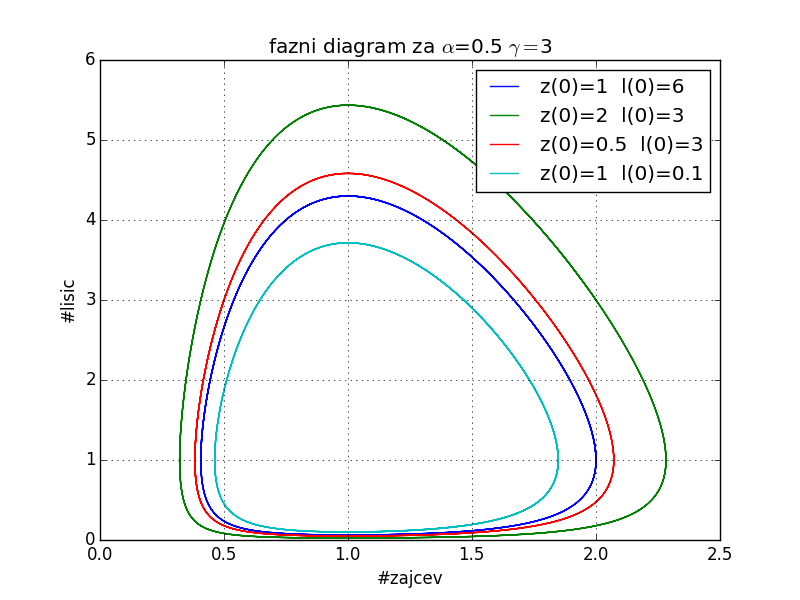
\includegraphics[scale=0.4]{slike/fazni-diagram-konstantna-alfa-gama.png}
%\caption{Druga stacionarna točka}
\end{minipage}%
}
\caption{Primeri faznih diagramov}
\end{figure}


\subsection{Frekvenčna odvisnost}
Oglejmo si kako se spreminja perioda spreminjanja populacije pri spreminjanju začetnih pogojev ene izmed populacije-graf \ref{fig:prva}.

\begin{figure}[h!]
%\centering
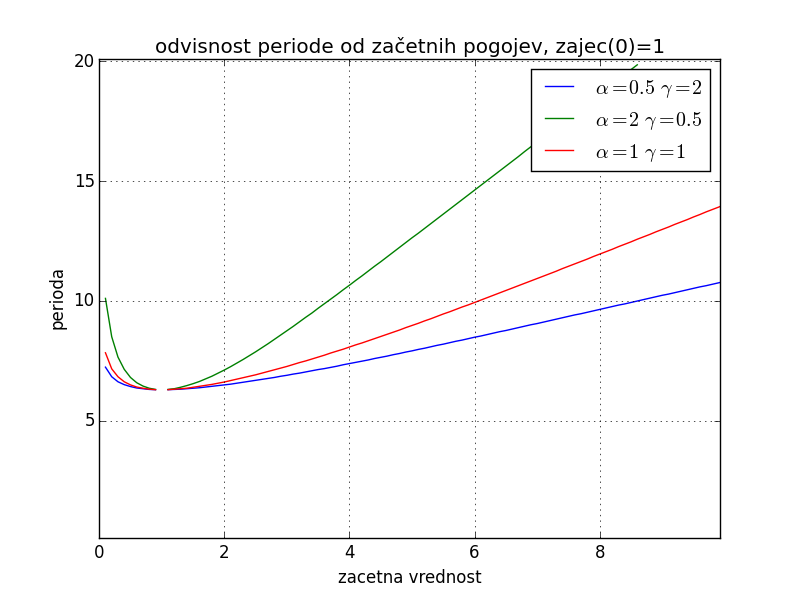
\includegraphics[scale=0.6]{slike/frekvencna_odvisnost.png}
\caption{Graf prikazuje spreminjanje periode, pri spreminjanju začetnih pogojev. Najbolj optimalno je imeti čim manjšo frekvenco spreminjanja populacije, zato je najbolj primerno, da imamo na začetku število obeh populacij enako (tam je ima funkcija minimum).}
\label{fig:prva}
\end{figure}

\pagebreak
\section{Laser}
Sedaj raziščimo populacijski model laserja. V laserju imamo atome, ki jih z zunanjim virom vzbujamo v višje stanje, pri tem pa del atomov spontano seva fotone. Število atomov označimo z $A$ ter število fotonov s $F$. Procese v laserju zapišemo:
\begin{equation}
\label{eq-laser-osnovna}
\begin{aligned}
\dot{A}&=r -p A (F+1) \\
\dot{F}&= \frac{F}{p} (A-1)
\end{aligned}
\end{equation}
Imamo konstantno črpanje atomov v vzbujeno stanje s hitrostjo $r$, ter parameter $p$, ki je razmerje fotonskih in spontanih atomskih izgub v laserju.
\subsection{Stacionarne točke}
Podobno kot v prejšnjem primeru enačbi \ref{eq-laser-osnovna} enačimo s $0$. Sledijo stacionarne točke $(A,F)$:
\begin{itemize}
\item $(A,F)=(1,\frac{r}{p}-1)$
\item $(A,F)=(\frac{r}{p},0)$
\end{itemize}
Iz prve točke vidimo, da mora biti $r>p$, saj imamo potem število fotonov pozitivno (število fotonov ne more biti negativno). Mejni primer, ko nimamo proizvodnje fotonov je: $r=p$. V drugem primeru nimamo proizvodnje fotonov, saj je število fotonov vedno enako nič.


\begin{figure}[h]
\noindent\makebox[\textwidth][l]{%
\hspace{-\dimexpr\oddsidemargin+1in}%

\begin{minipage}[t]{0.5\paperwidth}
\begin{flushleft}

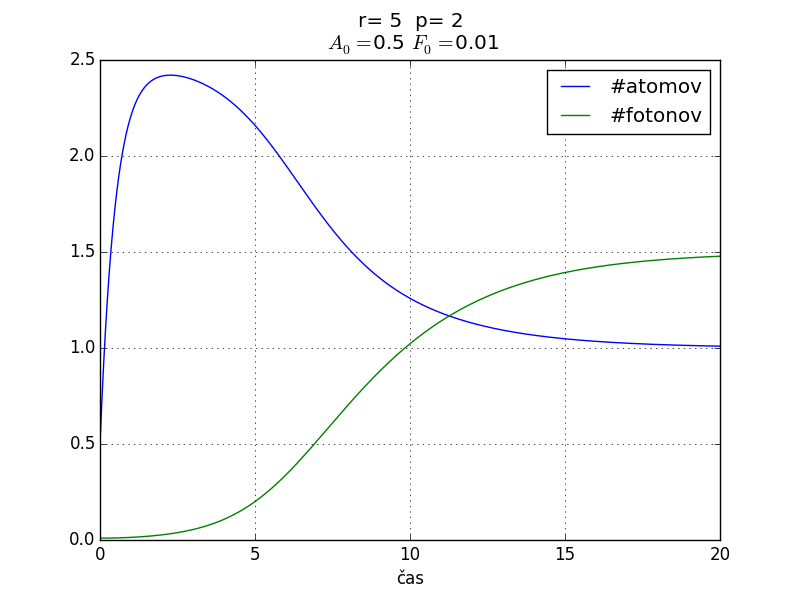
\includegraphics[scale=0.5]{slike/r=_5__p=_2___A_0=_0_5__F_0=_0_01.png}
\hspace{\fill}
\end{flushleft}
\end{minipage}
\begin{minipage}[t]{0.5\paperwidth}
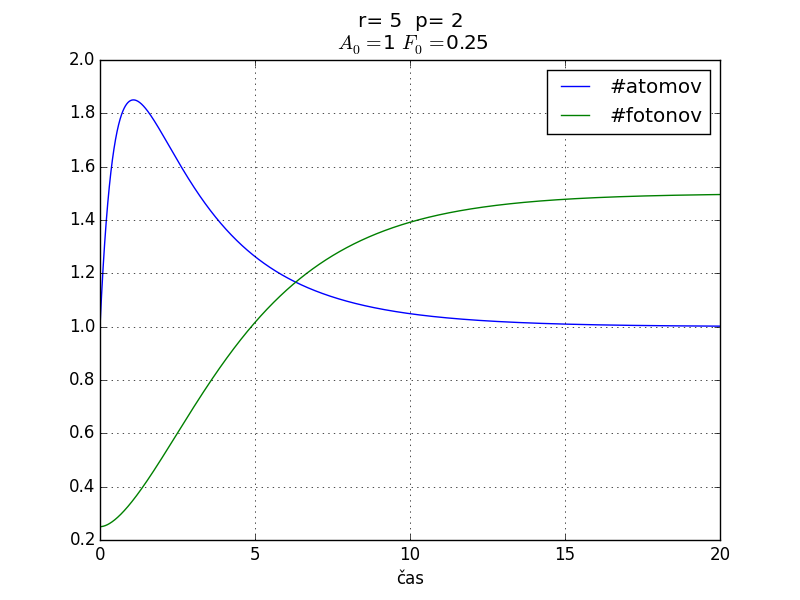
\includegraphics[scale=0.5]{slike/r=_5__p=_2___A_0=_1__F_0=_0_25.png}
\end{minipage}%
}
\noindent\makebox[\textwidth][l]{%
\hspace{-\dimexpr\oddsidemargin+1in}%

\begin{minipage}[t]{0.5\paperwidth}
\begin{flushleft}
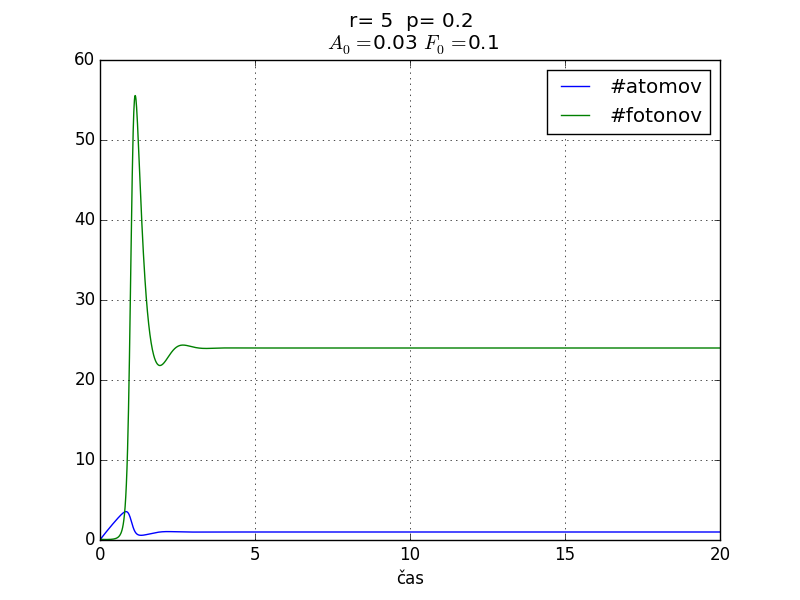
\includegraphics[scale=0.5]{slike/r=_5__p=_0_2___A_0=_0_03__F_0=_0_1.png}
\hspace{\fill}
\end{flushleft}
\end{minipage}
\begin{minipage}[t]{0.5\paperwidth}
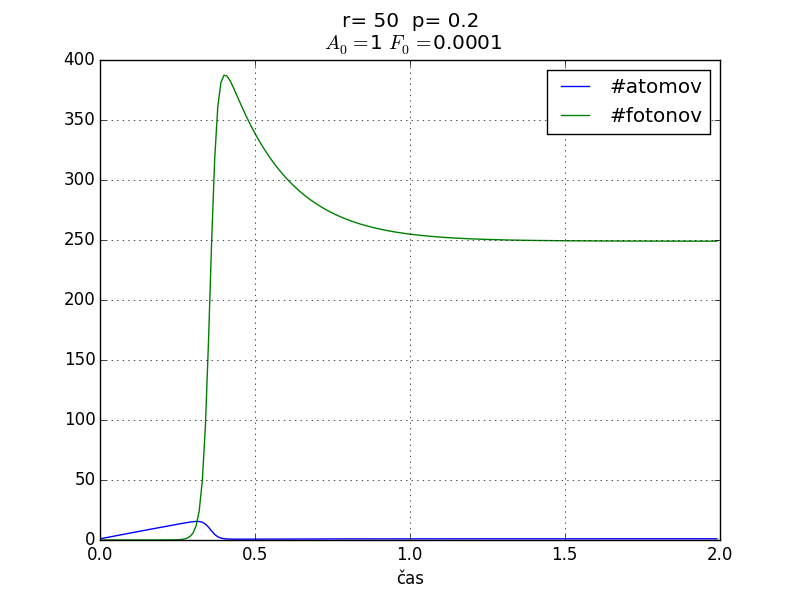
\includegraphics[scale=0.5]{slike/r=_50__p=_0_2___A_0=_1__F_0=_0_0001.png}
\end{minipage}%
}
\caption{Primeri rešitev za nekaj različnih začetnih pogojih in parametrov.}
\label{resitve-graf-laser-osnovne}
\end{figure}
\pagebreak


\section{Epidemija}
Oglejmo si še primer pri epidemiji. Populacijo razdelimo v tri skupine: D-dovzetni (osebe, ki lahko zbolijo),O-okuženi (osebe, ki so zbolele) ter I-imuni (cepljeni, osebe, ki ne morejo zboleti). Predpostavimo, da se skupna populacija ne zmanjšuje (zbolele osebe ne umrejo). Zapišemo enačbe:

\begin{equation}
\label{eq-epidemija-osnovna}
\begin{aligned}
\dot{D}&=- \alpha D O \\
\dot{O}&= \alpha D O - \beta O \\
\dot{I}&= \beta O
\end{aligned}
\end{equation}
Pri čemer nam parametra $\alpha$ in $\beta$ povesta, kako hitro prehajajo osebe iz dovzetnih v okuženo oz. iz okuženih v imune (ko enkrat ozdraviš, si imun na bolezen). 


\begin{figure}[h]
\noindent\makebox[\textwidth][l]{%
\hspace{-\dimexpr\oddsidemargin+1in}%

\begin{minipage}[t]{0.5\paperwidth}
\begin{flushleft}

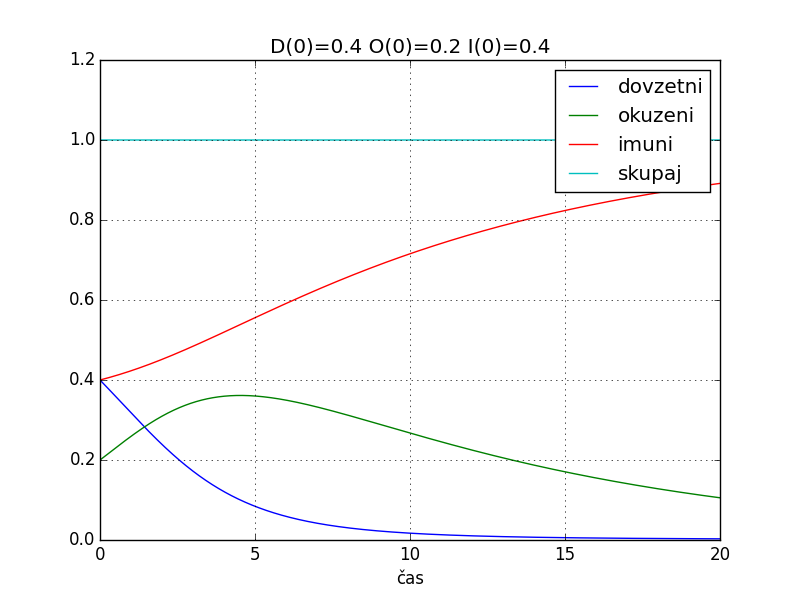
\includegraphics[scale=0.5]{slike/D(0)_0_4_O(0)_0_2_I(0)_0_4.png}
\hspace{\fill}
\end{flushleft}
\end{minipage}
\begin{minipage}[t]{0.5\paperwidth}
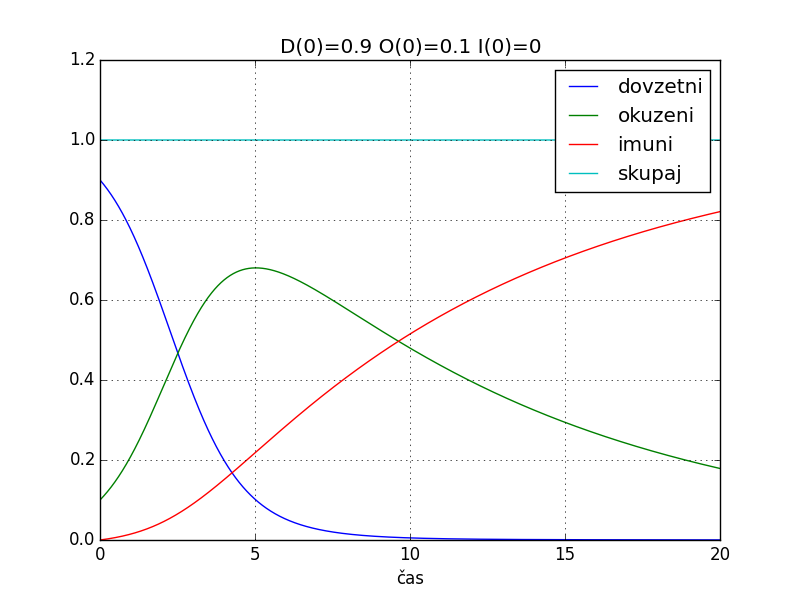
\includegraphics[scale=0.5]{slike/D(0)=0_9_O(0)=0_1_I(0)=0.png}
\end{minipage}%
}
\caption{Primera rešitev sistema enačb \ref{eq-epidemija-osnovna}. Parametra: $\alpha=1$, $\beta=0.1$}
\end{figure}
\pagebreak
\subsection{Vrh epidemije}
Pri epidemijah je pomembno, da se v bolnišnicah pripravijo na epidemijo. Oglejmo si kdaj pride vrh epidemije in koliko populacije bo zbolelo v odvisnosti od začetne imunosti populacije.

\begin{figure}[h]
\noindent\makebox[\textwidth][l]{%
\hspace{-\dimexpr\oddsidemargin+1in}%

\begin{minipage}[t]{0.5\paperwidth}
\begin{flushleft}

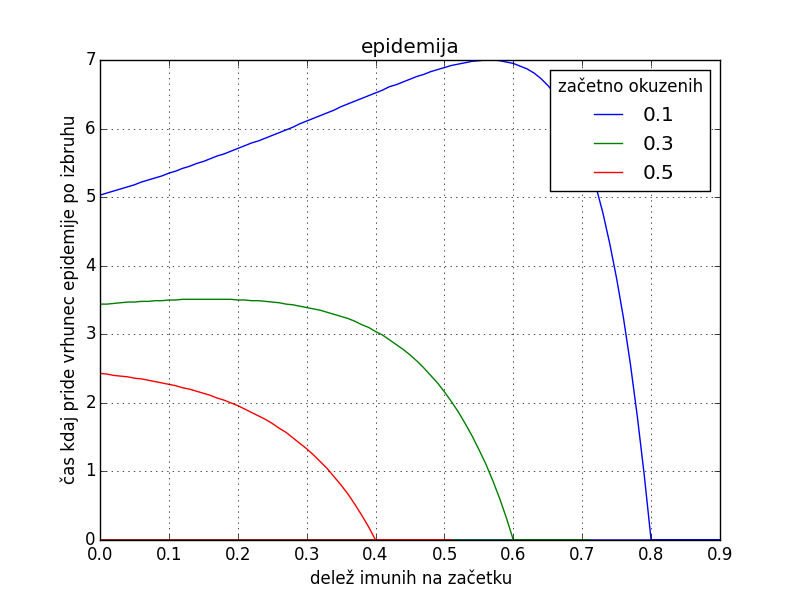
\includegraphics[scale=0.5]{slike/potreben_cas_postelje.png}
\hspace{\fill}
\end{flushleft}
\end{minipage}
\begin{minipage}[t]{0.5\paperwidth}
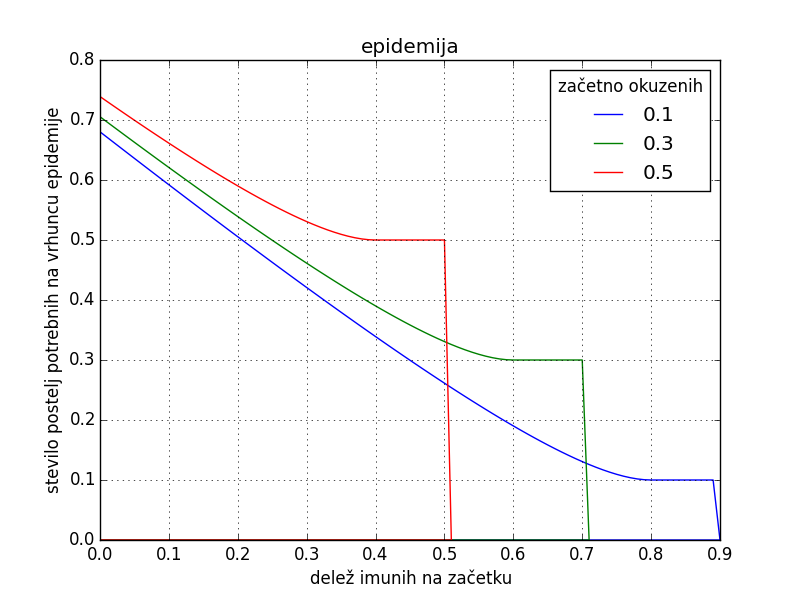
\includegraphics[scale=0.5]{slike/potreben_postelje.png}
\end{minipage}%
}
\caption{Graf kdaj pride do vrha epidemije in koliko močan bo vrh epidemije.}
\end{figure}
Opazimo, da bo vrh epidemije prišel prej, če bo na začetku več okuženih oseb v populaciji. Rezultat je smiseln. Prav tako bo vrh epidemije močnejši, če bo na začetku več okuženih.


\end{document}
